\documentclass[12pt, letterpaper] {article}
\usepackage{graphicx} % Required for inserting images
\usepackage[utf8]{inputenc}
\usepackage[margin=1in]{geometry}
\usepackage{amsmath}
\usepackage{hyperref}
\usepackage{graphicx}
\usepackage{caption}
\setlength{\parindent}{0em}
\setlength{\parskip}{0.5em}

\title{Assignment 3}
\author{Haobo Yuan}
\date{May 2024}

\begin{document}

\maketitle

\section{Question 1:}

In tackling this problem, our objective is to identify \( c \) values that converge towards a significant locus in the complex plane. To begin with, we must establish the function. As per the given problem statement, the boundary limit is defined by \( |z|^2 = \Re(z)^2 + \Im(z)^2 \). Consequently, any value falling below this threshold of \( |z|^2 \) can be deemed a convergence point.

\begin{figure}[h!]
    \centering
    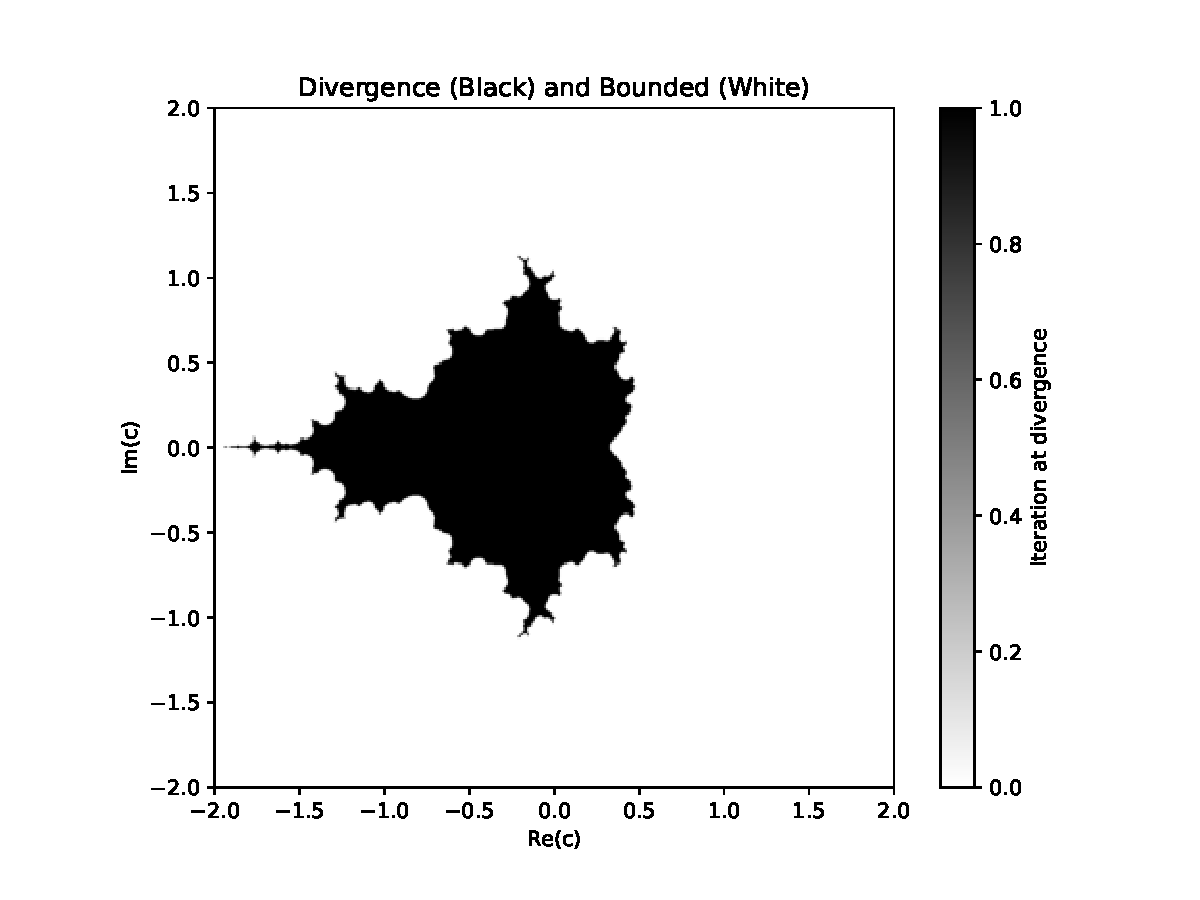
\includegraphics[width=0.5\linewidth, keepaspectratio]{Q1_figure_1.pdf}
    \caption{The colored graph illustrates the convergence of points in the complex plane.}
    \label{fig:Divergence (Black) and Bounded (White)}
\end{figure}

Moreover, it's essential to impose an iteration constraint on this function. By imposing a maximum iteration limit, we ensure that the function halts after reaching a predetermined number of steps. This prevents the function from running indefinitely and offers a practical means to ascertain convergence within a finite time frame.

Interestingly, a substantial maximum iteration count isn't necessary, as convergence is achieved rapidly across all points. This is evident from the second graph, titled "Iteration Number at Divergence."

\begin{figure}[h!]
    \centering
    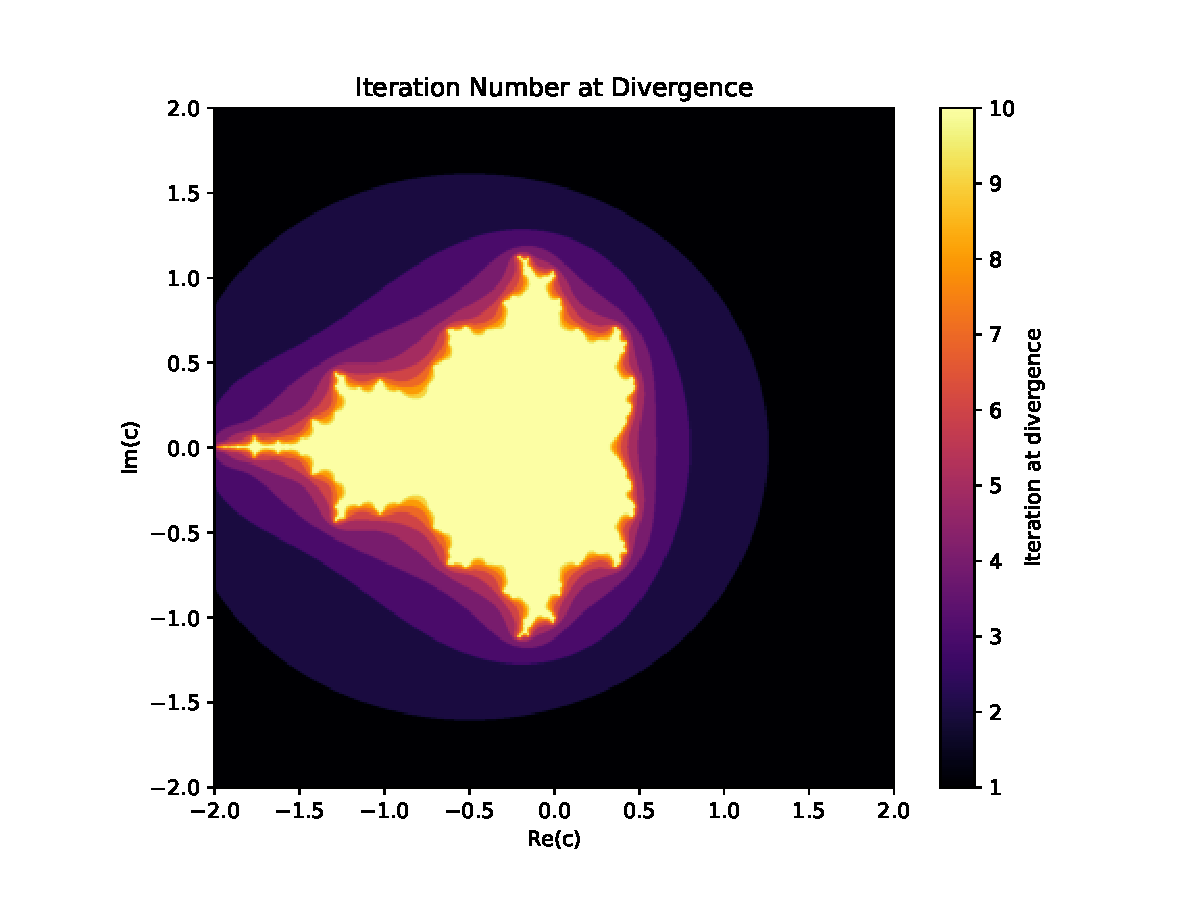
\includegraphics[width=0.5\linewidth, keepaspectratio]{Q1_figure_2.pdf}
    \caption{The colored graph indicates the number of iterations required for each point to converge, with a maximum iteration set at 10.}
    \label{fig:Iteration Number at Divergence}
\end{figure}

\section{Question 2:}

"A tornado's exact formation time and path can be influenced by minor perturbations, such as a distant butterfly flapping its wings several weeks earlier. " -- Lorentz 

The Lorenz Attractor, more commonly known as the "Butterfly Effect," was first introduced by Edward N. Lorenz in 1962. The equations describing this phenomenon, commonly referred to as Lorenz's equations (specifically equations 25, 26, and 27), are as follows:

\begin{eqnarray}
\dot X &=& -\sigma(X-Y)\\
\dot Y &=& rX -Y - XZ\\
\dot Z &=& -bZ + XY
\end{eqnarray}


Starting with the Lorentz system, there are various methods available for solving its differential equations. One approach I've opted for is employing solve\_ivp. As usual, we need to define a function called Lorentz which includes all three differential equations. By utilizing the same initial conditions as Lorentz, which are $W_0=[0., 1., 0.]$ and his parameter values [$\sigma, r, b$] = [10., 28, 8./3.]. we observe that these differentials exhibit chaotic (unpredictable) motion over time.

\begin{figure}[h!]
    \centering
    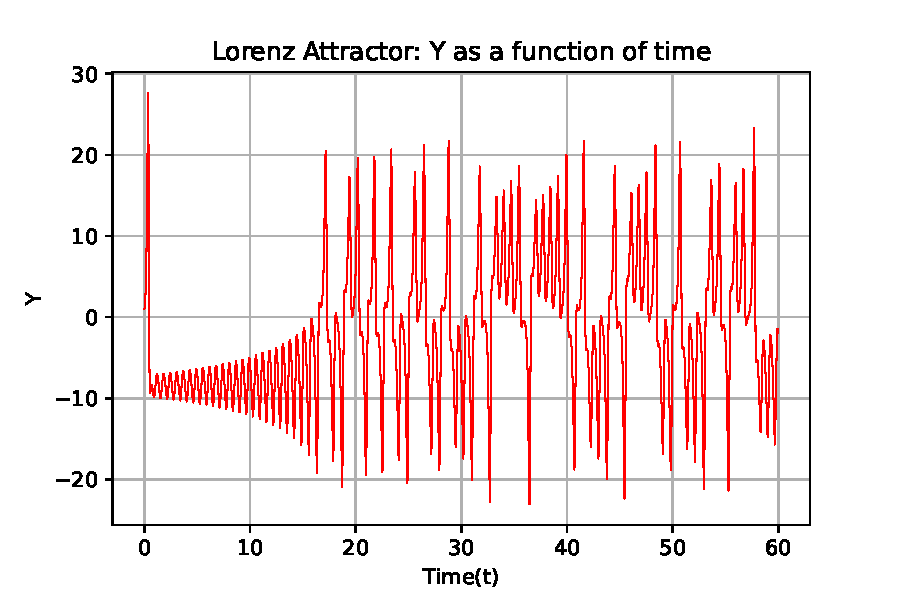
\includegraphics[width=0.45\linewidth, keepaspectratio]{Q2_figure_1.pdf}
    \caption{time from 0 to 60 with space of 0.01}
    \label{fig:Lorenz Attractor: Y as a function of time}
\end{figure}

Additionally, when plotting the graph in 2D, specifically in the Y Z (Figure 4.) and X Y (Figure 5.) planes, we obtain a figure resembling the shape of an 8 but it never repeats itself.

\begin{figure}[h!]
    \centering
    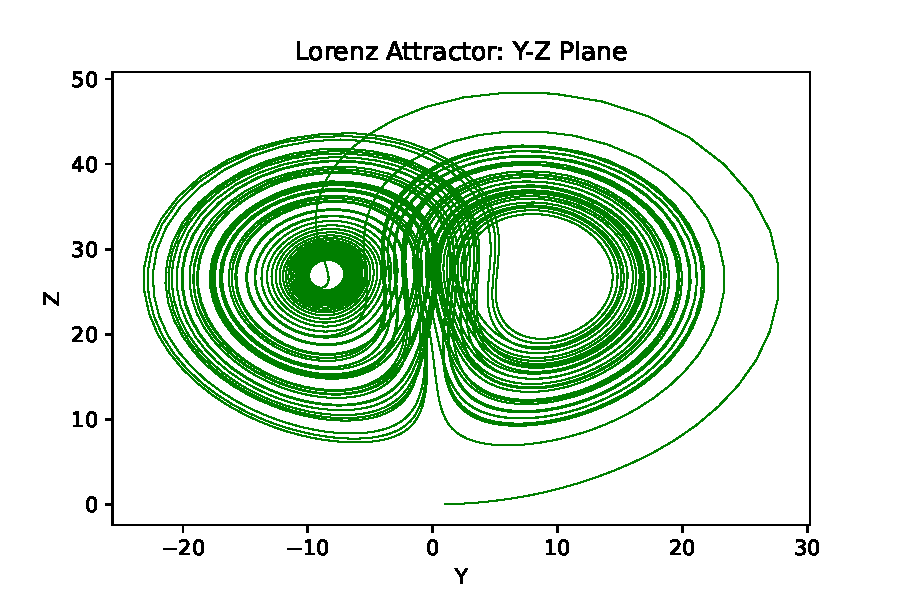
\includegraphics[width=0.5\linewidth, keepaspectratio]{Q2_figure_2_1.pdf}
    \caption{Lorentz Attractor in 2D Y - Z Plane}
    \label{fig:Lorenz Attractor: Y-Z Plane}
\end{figure}

\begin{figure}[h!]
    \centering
    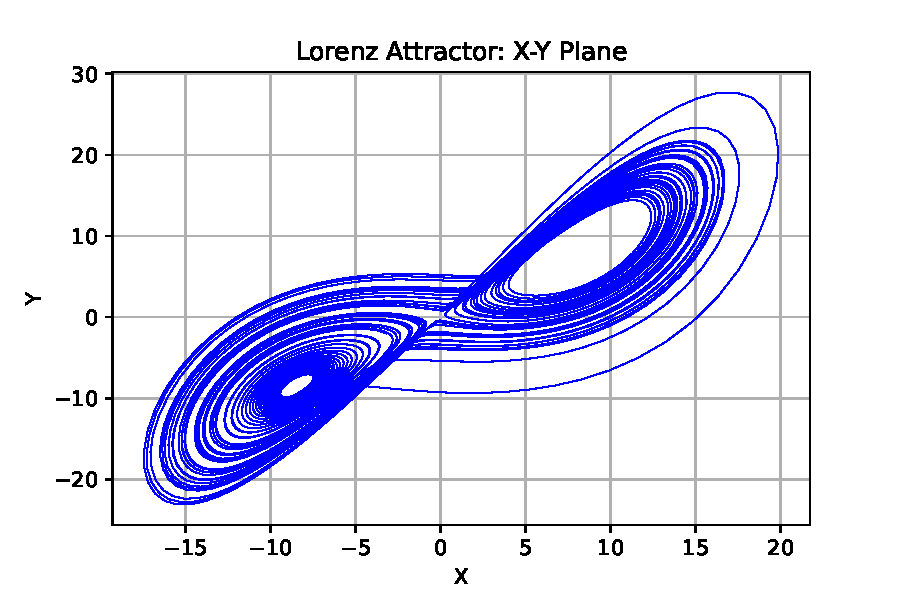
\includegraphics[width=0.5\linewidth, keepaspectratio]{Q2_figure_2_2.pdf}
    \caption{Lorentz Attractor in 2D X - Y Plane }
    \label{fig:Lorenz Attractor: Y-Z Plane}
\end{figure}

\clearpage
For a more comprehensive understanding of this shape, we can explore a 3D graph as Figure 6.

\begin{figure}[h!]
    \centering
    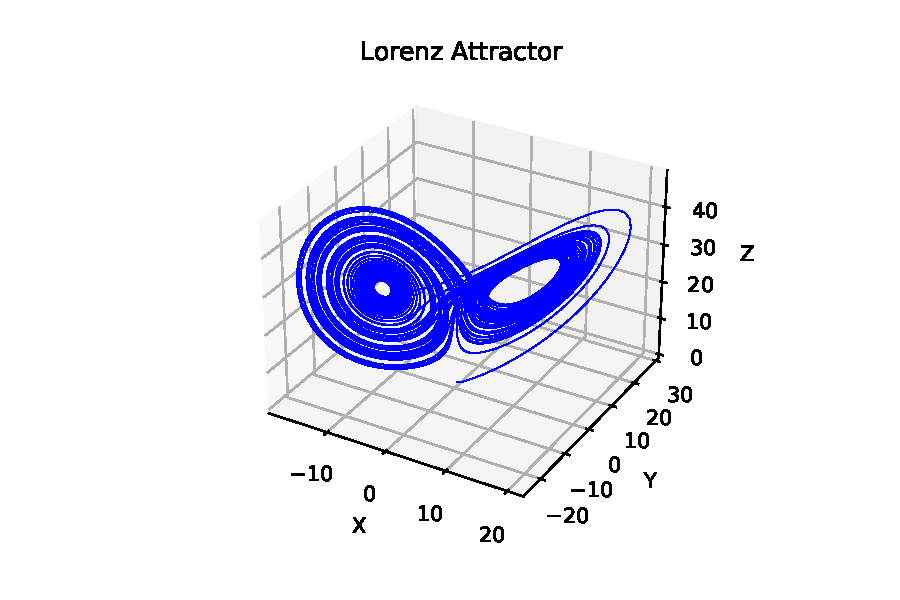
\includegraphics[width=0.5\linewidth, keepaspectratio]{Q2_figure_3.pdf}
    \caption{Lorentz Attractor in 3D }
    \label{fig:Lorenz Attractor 3D}
\end{figure}


We can also see what happend if we change the initial condition with a small step, that is $W_new = [0., 1.e-8, 0.]$ the graph as Figure 7.

\begin{figure}[h!]
    \centering
    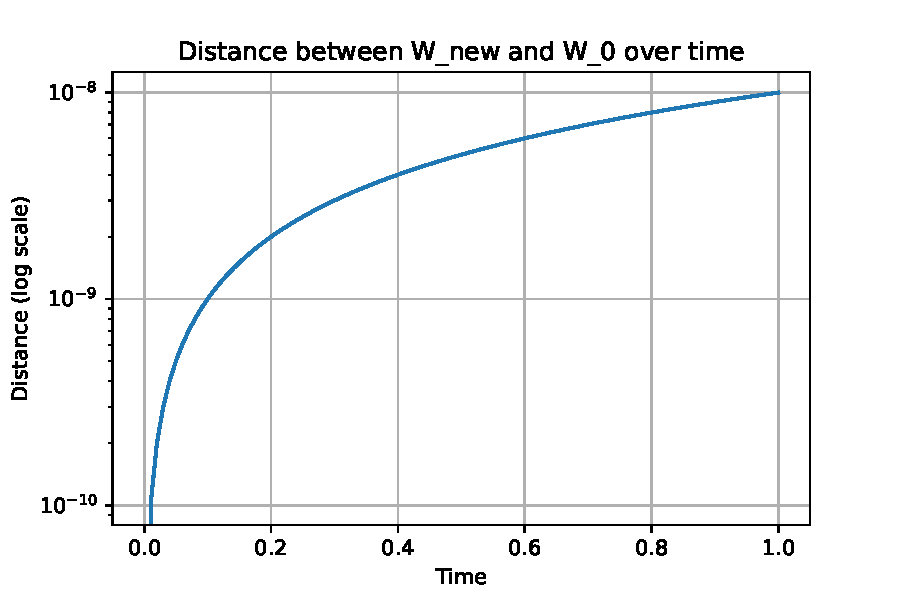
\includegraphics[width=0.5\linewidth, keepaspectratio]{Q2_figure_4.pdf}
    \caption{The distance between \( W_{\text{new}} \) and \( W_0 \) changes rapidly over time, even when starting with a very small difference. This phenomenon highlights the sensitivity of the system to initial conditions.}
    \label{fig:Distance between W_new and W_0 over time}
\end{figure}



\section{Conclusion:}

The characteristic butterfly-shaped orbits of the Lorenz attractor illustrate the chaotic nature of the system. The trajectory never settles into a fixed point or a periodic orbit, reflecting the sensitivity to initial conditions that is a hallmark of chaotic systems.


\end{document}
